\chapter{Methods and Results}\thispagestyle{fancy}
\paragraph*{}
Now we are equipped sufficiently to go deeper into our main topic of random Boolean networks and, more precisely, some statistical observations of their attractors and their stability behavior. Even though the previous chapter was said to be the theoretical background, we will onwards from here still encounter many theoretical aspects and derivations. In scientific research, there is no strict division between theory and observation. It is more like an interplay between those two aspects, as it has also been for us and the random Boolean networks the case.


\paragraph*{}
Random boolean networks (RBN) are discrete models where such attractors appear and due to their finitely large state space can accessibly be studied. They were first proposed by C. C. Walker and William Ross Ashby in 1966 \cite{walker1966temporal}, but got popularized by Stuart A. Kauffmans work in 1969, who wanted to model and understand gene regulatory networks \cite{kauffman1969homeostasis}. Over the years boolean networks have been used to model a wide variety of complex systems and their dynamics from many different fields such as social systems \cite{moreira2004efficient}, neural networks \cite{rosen2001multilayer} and the previously mentioned gene regulatory networks.

\paragraph*{}
All kinds of different models have been proposed and studied over time, e.g. using a certain type of network structure like in \cite{aldana2003boolean2}, \cite{iguchi2007boolean} and \cite{serra2004dynamics}, where they used scale-free degree distributions or choosing only canalizing coupling functions like in \cite{moreira2005canalizing}. Real gene regulatory networks have been showing some evidence for both approaches being reasonable (see \cite{moreira2005canalizing} and \cite{shaw2003evidence}).

\paragraph*{}
Since our main research interest lies in understanding the properties of attractors as such and not only compared to gene regulatory networks, we will stick to the classically proposed Kauffman-Network as our RBN. To avoid uncertainties we define our model in the following subsection and explain all necessary terms.


\section{Topological Properties}

\paragraph{}
Before starting investigations on any computational model, one has to make sure that the own implementations are correct and reproduce some already known properties. So we started by generating a few Kauffman-Networks and looked at their out-degree as our random variable $X=k^{(out)}$. The Poisson approximation presented in equation (\ref{eq:Poisson}) was what we were interested in checking first and it appears to be fairly good. It becomes even better for larger $N$ and smaller $ p = K/N $ as can be seen in Figure \ref{fig:Poisson}. 

\begin{figure}
	\includegraphics[width=\textwidth]{Plots/poisson_distributed}
	\caption{Three randomly created Kauffman-Networks with differing $N$ and $K$. The gray bars show the ratio the nodes with an out-degree of $k$ had compared to all others. The Poisson approximation (red, equation (\ref{eq:Poisson})) is a little off for the network on the right. But for the other two it appears to be pretty good.}
	\label{fig:Poisson}
\end{figure}

\paragraph*{}
The in-degree is due to the definition of the Kauffman-Network always $k^{(in)}=K$. Via the construction of choosing $K$ different nodes for every single node, this is guaranteed to be the case. 

\paragraph*{}
We started our studies of random boolean networks by recreating some known results to make sure our implementations work just as expected. Therefore we created networks with $N$ vertices and edges that would result in a constant $K=k^{(in)}$ and a Poisson distributed $k^{(out)}$. The results of our first attempts can be seen in Figure \ref{fig:phase_behavior} and recreate the long term behavior of RBNs in terms of their ability to propagate information in their different phases or instead how differences between states grow over time. We will explain this in the following in much more detail.

\section{Dynamics and Phases}
\paragraph*{}
Random Boolean Networks exhibit different behavior depending on the graph structure that is used. From the viewpoint of information flow, they can either retain or lose memory. The easiest way to see this is with a mean-field approximation of the $N $-$K $ model with magnetization bias $p$. It means we will not look at individual node behavior and instead focus on averages over the whole system. For this, we will always assume a large number of vertices $N\longrightarrow\infty$ in this section.

\paragraph{Mean-Field Approximation}
Let us say we have two different initial conditions $\Sigma_0$ and $\tilde{\Sigma}_0$. Their Hamming distance $D(0)$ can be calculated accordingly to equation (\ref{eq:hamming_distance}) and gives the number of elements that are different in these two states. A single node influences averagely $K$ other ones, thus $KD(0)$ coupling functions get affected in the next time step. There are two possible ways of having them be different, each with a probability of $p(1-p)$. In total this means that for the next time step the distance grows as $D(1) = 2p(1-p)KD(0)$. After the time $t$ it will recursively become:
\begin{equation}
D(t) = \left[2p(1-p)K\right]^t D(0) = D(0)e^{t\ln[2p(1-p)K]}.
\end{equation}
There are now three different things that can happen with such an equation. It can grow exponentially, go to zero or stay just the same, which happens if 
\begin{equation}\label{eq:critical_condition}
2p(1-p)K=1.
\end{equation}
Thus for a given magnetization bias $p$, the tipping point, where the system changes its behavior, also just called its critical connectivity, is at 
\begin{equation}\label{eq:critical_connectivity}
K_c = \frac{1}{2p(1-p)}.
\end{equation}
\paragraph*{}
Also, the other way around, if we fix $ K $ the critical bias for the coupling functions can be calculated by:
\begin{equation}\label{eq:critical_magnetization_bias}
p_c^{\pm}=\frac{1}{2}\pm \sqrt{\frac{1}{4}-\frac{1}{2K}}.
\end{equation}

\begin{figure}
	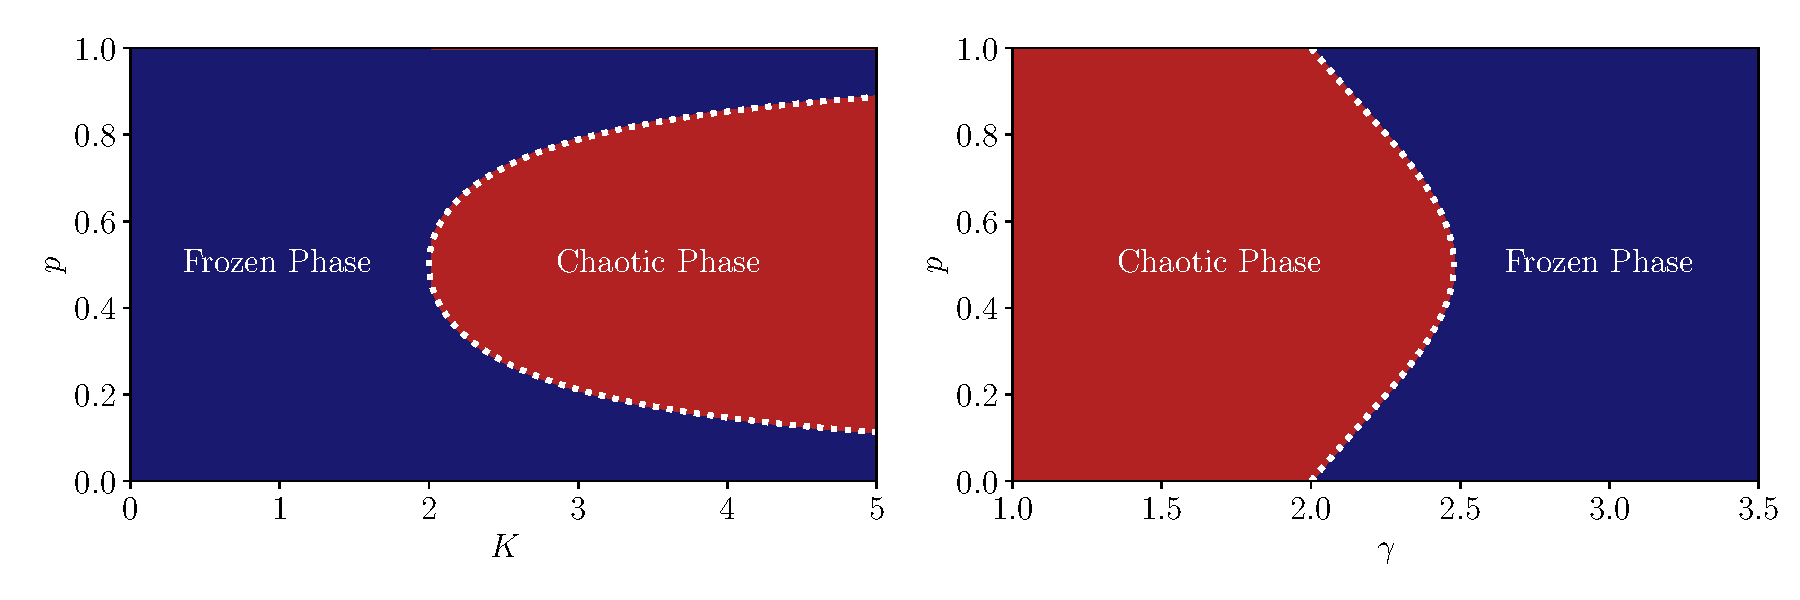
\includegraphics[width=\textwidth]{Plots/network_phases}
	\caption{Here we have the phase diagrams of different RBN models, with the magnetization bias $p$. Left: $N$-$K$ model, where the second parameter is the connectivity $K$. Right: Scale-free model, with the scaling parameter $\gamma$. }
	\label{fig:network_phases}
\end{figure}


\paragraph{}
In the context of the RBN, this means we have the following different phases:
\begin{itemize}
	\item[-] Frozen ($K<K_c$): The Hamming distance decreases over time and the two initially different states will most likely end up in the same configuration. It often coincides with the arrival at a fixpoint, which means the nodes stop changing over time, which is why this phase is called frozen. This means we lose all the initial information on the systems we had at the beginning over time.
	\item[-] Critical ($K=K_c$): At this point, the distance stays roughly the same according to the mean-field approximation. But since it only works on averages, the system's fluctuations at the critical value are not considered.
	\item[-] Chaotic ($K>K_c$): The different initial conditions diverge exponentially over time. Of course, with only a finite number of nodes $ N $, the difference between the two initial configurations can never get any larger than this. Thus, at every time step $t$, it will be $D(t) \leq N $, which is again something that the mean-field approximation does not account for.
\end{itemize}

\paragraph{}
Since we arrived at the critical condition in equation (\ref{eq:critical_condition}) only by looking at averages, the same argumentation also holds for scale-free networks. We only need to calculate the average out-degree and can do this by using the probability distribution given in equation (\ref{eq:scale_free_degree_distribution}):
\begin{equation}
K = \langle k^{(out)}\rangle = \sum\limits_{k=1}^{\infty}kp_k^{(out)} = \frac{1}{\zeta(\gamma)}\sum\limits_{k=1}^{\infty}k^{1-\gamma} =
\begin{cases}
	\infty                                & \text{if } 1 < \gamma \leq 2, \\
	\frac{\zeta(\gamma-1)}{\zeta(\gamma)} & \text{if } 2 < \gamma .
\end{cases}
\end{equation}

\paragraph*{}
Now we can solve for the critical magnetization bias with equation (\ref{eq:critical_magnetization_bias}). With this, we can create the transition curve of the phase diagrams for the $N$-$K$ model and scale-free networks, which we can see in Figure \ref{fig:network_phases}.

\paragraph*{}
\begin{figure}
	\begin{subfigure}{\textwidth}
		\includegraphics[width=\textwidth]{Plots/phase_behavior}
		\label{fig:sfig1.1}
	\end{subfigure}
	\caption{Here we reproduced some known classical results, as Aldana et al. have shown in their review \cite{aldana2003boolean2}. Both graphs show the normalized Hamming distance with respect to time for networks with $ N=10000 $ and $ K=4 $. The left is for the $ N $-$ K $ model and the right is for a square lattice with periodic boundary conditions. The simulation started at a random state and used as the comparison state the same one with $ 100 $ nodes flipped. We varied the bias between values from $ p_1 = 0.05 $ to $ p_10 = 0.275 $ and averaged for every one of them over $ 1000 $ network realizations.}
	\label{fig:phase_behavior}
\end{figure}

\paragraph*{}
We ran some simulations and measured the normalized Hamming distance for two states of the $N$-$K$ model and square lattice networks, which started with $1\%$ of their node values being different. The results can be seen in Figure \ref{fig:phase_behavior}. We got the idea for doing this from the work of M. Aldana et al. \cite{aldana2003boolean2}, though there can be found many other authors throughout the literature that also already did the same.

\paragraph*{}
The $N$-$K$ model is the one that shows the behavior we described just above. In the chaotic phase, the differences between the two states grow over time. Near the critical line at $ p_c = \tfrac{\sqrt{2}-1}{2\sqrt{2}} \simeq 0.1464 $ the amount of flipped vertices stays roughly the same. For networks in the frozen phase, the overwhelming majority of states tend to evolve into the same fixpoint and this only in a few steps.

\paragraph*{}
The square lattice networks, on the other hand, show somewhat different behavior. M. Aldana et al. \cite{aldana2003boolean2} give a value for the critical bias of around $p_c\approx 0.27$. However, as we can clearly see, the distance already retains or even grows with time for much smaller values. Moreover, the window from smallest to greatest bias is much more narrow to what we have seen before by direct comparison. This has to do with the high order of symmetry the underlying network possesses. The main takeaway from this could be that the underlying graph plays a significant role in random boolean networks' behavior.

\paragraph*{Annealed Approximation}\label{sec:annealed_approximation}
The previous mean-field approximation already delivered some exciting results, which are also in agreement with computational observations. But the argumentation appears to be quite rough and, as we mentioned above, can not account for any fluctuations in the system. Thus, we will look at another approximation, which can be done a little more rigorously and provides methods to observe additional properties.

\paragraph*{}
B. Derrida and Y. Pomea \cite{derrida1986random} presented in 1985 a new way to calculate several quantities of random boolean networks, which they called the annealed approximation. The name is an analogy from the field of spin glasses, where it means that certain random variables of the system can change over time. In the same language, all the models we have presented so far would be quenched since once we decided on the network structure and the boolean functions, those become permanent. In contrast to this, they can change at every time step in the annealed approximation. By this, they lose their correlation to the previously given boolean functions. The system also becomes non-deterministic and thereby, no attractors or related structured will appear any longer. But for large enough systems, where $N\longrightarrow\infty$, they will only play a secondary role anyway.

\paragraph*{}
The derivations we are making here are in the spirit of the original work from B. Derrida and Y. Pomea. We start again by considering two random different initial states $\Sigma_0$ and $\tilde{\Sigma}_0$ for a given random boolean network, that have a Hamming distance of $D(0) = n > 0$. The system has a large number of nodes $N$ and the coupling constant $K$. The nodes can be divided into two sets, the ones that are different $A$ and those that are the same in both states $B$. Only if a node takes input nodes from set $B$ it can have a different outcome for its value in $\Sigma_1$ and $\tilde{\Sigma}_1$. We now want to consider the odds that $N_0$ nodes only take their inputs from $A$. The probability for a single vertex to draw $K$ times only from $A$ is:
\begin{equation}\label{eq:draw_from_one_set}
q = \prod\limits_{i = 0}^{K-1}\frac{N-n-i}{N-i} \approx \left(\frac{N-n}{N}\right)^K.
\end{equation}
The right hand side is a good approximation for very large $N$ and only finitely large $K$. With this, we see that this is again a Bernoulli process and with equation (\ref{eq:Bernoulli}) we can calculate the probability distribution for $N_0$ to be:
\begin{equation}
Q(N_0) = {N \choose N_0} \left[\left(\frac{N-n}{N}\right)^K\right]^{N_0}  \left[1-\left(\frac{N-n}{N}\right)^K\right]^{N-N_0}.
\end{equation}

\paragraph*{}
If the nodes do take input from set $B$, the probability that they will be different in the next time step will be again $2p(1-p)$. This is all we needed to calculate the likelihood that we will have $m$ different nodes after a single time step:
\begin{equation}
\begin{split}
P_1(m) &= \sum\limits_{N_0 = 0}^{N-m} {N-N_0 \choose m} Q(N_0) \tilde{p}^m (1-\tilde{p})^{N-N_0-m} \\
&= \sum\limits_{N_0 = 0}^{N-m} \frac{(N-N_0)!}{m!(N-N_0-m)!}\frac{N!}{N_0 !(N-N_0)!} q^{N_0}  (1-q)^{N-N_0} \tilde{p}^m (1-\tilde{p})^{N-N_0-m}\\
&= {N \choose m} \left[\tilde{p}(1-q)\right]^m \cdot\sum\limits_{N_0 = 0}^{N-m} {N-m \choose N_0} q^{N_0}  \left[(1-q) (1-\tilde{p})\right]^{N-m-N_0}\\
&= {N \choose m} \left[\tilde{p}(1-q)\right]^m \left[1-\tilde{p}(1-q)\right]^{N-m}.
\end{split}
\end{equation}
This is a very nice result since it shows us that we have, in fact, again a binomial distribution with the individual probability of a single event to occur of $\tilde{p}(1-q)$. We could have also guessed that this must be the case since this is nothing else than the probability for a single node to be chosen from the set of nodes with unequal values and, at the same time, having functions that provide different outcomes. Nonetheless, it is good to see that after a short derivation, we end up with a clean and intuitive result. In their work, B. Derrida and Y. Pomea arrive at this equation in a way where it is not immediately apparent that this is just a binomial distribution.

\paragraph*{}
Now we know from section \ref{sec:bernoulli_process} that the expected value will just be $E[X] = N\tilde{p}(1-q)$, if $X$ is the random variable representing all possible values of $m$. The standard deviation is, as we know, proportional to $ \sqrt{N} $, which is neglectable compared to the whole possible range of $ X $, since
\begin{equation}
\frac{\sqrt{N}}{N} \stackrel{N\rightarrow\infty}{\longrightarrow}0.
\end{equation}
We can conclude that the peak around the mean is incredibly narrow compared to all possible values and because of this, it will be almost surely: $m = N\tilde{p}(1-q)$. Introducing the variables $y_0:=n/N$ and $y_1:=m/N$ and resubstituting $\tilde{p}$ and $q$ lets us rewrite the equation into:
\begin{equation}\label{eq:first_map}
y_1 = 2p(1-p)[1-(1-y_0)^K]
\end{equation}

\paragraph*{}
As of right now, we would not have needed to introduce the annealed approximation since all our arguments are also valid in the quenched model. But this changes if we have to consider the next time step and all others after that up to $t$. To redo the equation's derivation (\ref{eq:first_map}) we would have to respect the correlations to the first chosen functions. But in the annealed model, every step stays the same as before and we arrive at:
\begin{equation}\label{eq:annealed_map}
y_{t+1} = 2p(1-p)[1-(1-y_t)^K] =: \phi(y_t).
\end{equation}

\paragraph*{}
It is obvious that $y^* = 0$ is a fixpoint of this map and by calculating the derivative at it, we will analyze its stability:
\begin{equation}
\phi'(0) = 2p(1-p)K
\begin{cases}
\leq 1 & \text{if } K \leq K_c, \\
> 1 & \text{if } K > K_c.
\end{cases}
\end{equation}

\paragraph*{}
The critical connectivity is the same as we had before in equation (\ref{eq:critical_connectivity}). We see that for values greater than $K_c$, zero becomes an unstable fixpoint. This is what we conclude when comparing the results with the definition of fixpoint stability in equation (\ref{eq:fixpoint_stability}). We arrive at the same result as we had in the mean-field approximation and observe a change of behavior for systems that cross $K_c$. In addition to that, we now have the map (\ref{eq:annealed_map}) from which we can deduce complementary information on networks, where we know their average connectivity $K$. Let us define the random variable $Y$ as the normalized distance between two consecutive time-steps. The expected value of it should now be in agreement with the stable fixpoint of $\phi$ and it certainly is in the chaotic phase, which we can see in Table \ref{tab:fixpoints}.

\paragraph*{}
\begin{table}[h!]
	\centering
\begin{tabular}{|c|C{1.5cm}|C{1.5cm}|C{1.5cm}|C{1.5cm}|}
	\hline
	\multicolumn{5}{|c|}{$N=10^3$, Ensemble Size: $10^4$,} \\ 
	\multicolumn{5}{|c|}{Measured between: $t_1 = 49$ and $t_2=50$} \\ 
	\hline
	$K$ & $p$ & $y^*$ & $E[Y]$ & $\text{Std}[Y]$ \\ 
	\hline\hline  
	\multirow{3}{*}{3} & $0.212$ & $0.002$ & $0.039$ & $0.035$ \\ 
	\cline{2-5}
	& $0.300$ & $0.223$ & $0.219$ & $0.034$ \\ 
	\cline{2-5}
	& $0.450$ & $0.345$ & $0.344$ & $0.024$ \\ 
	\hline\hline 
	\multirow{3}{*}{4} & $0.147$ & $0.002$ & $0.029$ & $0.027$ \\ 
	\cline{2-5} 
	& $0.300$ & $0.341$ & $0.340$ & $0.020$ \\ 
	\cline{2-5}
	& $0.450$ & $0.450$ & $0.450$ & $0.017$ \\ 
	\hline\hline  
	\multirow{3}{*}{5} & $0.113$ & $0.001$ & $0.024$ & $0.023$ \\ 
	\cline{2-5}
	& $0.300$ & $0.382$ & $0.382$ & $0.017$ \\ 
	\cline{2-5}
	& $0.450$ & $0.475$ & $0.475$ & $0.016$ \\ 
	\hline
\end{tabular} 
\vspace*{0.3cm}
\caption{The observed random variable $ Y $ is the change of the normalized Hamming distance (equation (\ref{eq:hamming_distance}) divided by $ N $) for an ensemble of $ 10^4 $ RBNs, each with $ 10^3 $ nodes and certain fixed $ K $'s and $ p $'s between the $ 49 $ and $ 50 $ time-step after a random initialization at $ t = 0 $. We calculated the expected value (\ref{eq:expected_value}) and the standard deviation (\ref{eq:standard_deviation}) for $ Y $, which we compare to the second fixpoint of the map (\ref{eq:annealed_map}).}
\label{tab:fixpoints}
\par
\end{table}

\paragraph*{}
We come to similar conclusions as B. Derrida and Y. Pomea did in their original work. The map in equation \ref{eq:annealed_map} gives a pretty useful description for networks in the chaotic regime, even though we derived it with the annealed approximation. Near the critical point, the results are not as close anymore.

\paragraph*{}
The approximation is good for understanding some aspects of random boolean networks, but not for all. It excludes by its definition the appearance of any attractors and is therefore not suited for studying everything related to them. However, we gained a good understanding of networks' behavior in their different phases and how small perturbations grow over time.

\section{Attractors}

\paragraph*{}
Now we come to one of the main subjects of investigations of this thesis. We were interested in finding out more about the basins of attraction of attractors and wanted to study their structure, sizes, and how this relates to the cycles' length. Moreover, we wanted to do this for systems in the different phases and compare them like this.

\paragraph*{}
To average over sufficiently large network ensembles, we had to develop an efficient way of fully analyzing the whole phase space of a single realization. There have already been ways to find the whole basin of attraction for a single already found cycle, like the one introduced by A. Wuensche \cite{wuensche1997attractor}. 

\paragraph*{}
However, one has to reverse engineer all the states a single state could arise from by checking all the possible input values for every node that would lead to the appropriate values. This assumes full knowledge of all boolean functions, which our solution does not. With our algorithm, we only need to know the next state for every single state in the phase space, making it more general and applicable to other models than random boolean networks. We basically have just to go through all the states once forwards and then backward and collect all the necessary information on the fly. The main idea for this stems from how list types are defined in the programming language $\texttt{C++}$. For more details on our algorithm, see the Appendix \ref{sec:algorithm}.

\paragraph*{}
\begin{figure}[t]
	\includegraphics[width=\textwidth]{Plots/basin_sizes_N14}
	\caption{Here we plotted attractor length $ L $ against the fraction the basin of attraction occupies compared to the whole phase space (normalized basin size). Those examples are representatives for the different phases of boolean networks. All their coupling functions have a bias of $ p = 0.5 $. Below those scatter plots, we see the probability distribution for a cycle to have length $ L $. The green triangles are the proportion of the phase space which are garden-of-Eden states. All ensembles were created over $ 10^6 $ network realizations and $ L_{max} $ is the longest attractor we could find in each of those sets.}
	\label{fig:basin_sizes_main}
\end{figure}

\paragraph*{}
Figure \ref{fig:basin_sizes_main} can be seen as a summary of some of our main findings. However, what we see in this graphic is far too rich and we will go through everything there is to notice in many more details in the following subsections. What can be obviously stated is that the size of the basins of attraction has wildly different behavior comparing networks in the frozen phase, on the critical line and in the chaotic phase.

\paragraph*{}
We can make a few remarks on the phases of random Boolean networks in general before we continue with the more detailed studies of the results. If you look at Figures \ref{fig:basin_sizes_main_additional_sizes} and \ref{fig:basin_sizes_main_additional_frozen_chaotic}, you can make the following two observations. First, the results we get for the averaged sizes of the basins of attraction are very similar for different network sizes. Here we only showed $N=10$ and $N=12$ as examples, but this is the case at least for networks between the sizes $N=6$ and $N=16$. For the larger networks, we created only fewer realizations. Thus we decided to only look at $N=14$ systems in Figure \ref{fig:basin_sizes_main} and not the larger ones.

\paragraph*{}
The second general observation we can make is that even though we can accurately calculate the critical values, the network ensembles' observed behavior seems to be rather gradually changing between similar connectivities $K$. If we look at an ensemble at sets with critical systems, it is not too hard to understand why we would find that it is like this. We use realizations where everything gets determined at the start with random probabilities. Thus we will have realizations that tend to be either in the frozen or chaotic phase, rather than only critical ones. 

\paragraph*{}
To construct an extreme case, we could think about a network, which got applied only with constant and fully canalizing coupling functions. Such a system is not too unlikely for smaller system sizes and is definitely one that belongs with its behavior to the frozen phase. Consider random couplings on top of the randomly chosen Boolean functions. Then, even for larger systems, there will also be a non-zero probability to create a realization that would rather belong to the frozen phase. Similarly, we could make this argument for systems that would rather belong in the chaotic phase.

\paragraph*{}
So, all in all, we have for $K=2$ a mixture of critical systems and those belonging to the frozen or chaotic phases. And depending on whether we choose coupling values below or above, we will get more of the one or the other in our ensemble data, which explains the gradual change between the values. 

\paragraph*{}
That criticality is still not only a mixture of frozen and chaotic systems can be seen by looking at the maximal lengths $L_{max}$ we could find in all three regions. They are longer in the chaotic phase than in the frozen one, which had to be expected. But the largest cycles we could find within ensembles of $10^6$ realizations happened for all system sizes to be around the critical value. There is no way to explain this observation with the previous explanation. Thus it means something special having critical RBNs, even if we do not look at them in the thermodynamical limit, at which we derive most notions of criticality in general.


\subsection{Garden-of-Eden States}
\paragraph*{}
Throughout the literature, one does not find too many works on the garden-of-Eden states, though they are regularly mentioned. One example would be the Ph. D. thesis of A. Wuensche \cite{wuensche1997attractor}, where he analyzed the G-density and the phase space in-degree for cellular automata (CA). Those are not the same as our RBNs, but they are closely related. One could say that CAs are basically RBNs with a grid structure as their network and every node gets applied with the same boolean function.

\paragraph*{}
\begin{figure}
	\includegraphics[width=\textwidth]{Plots/in_degree_N10}
	\centering
	\caption{Those are the in-degree distributions that we obtain by analyzing the state space of different network ensembles. For comparison, we draw on the right the distribution we get by randomly choosing the next time step out of all $2^{14}$ possible states.}
	\label{fig:in-degree}
\end{figure}

\paragraph*{}
We already introduced the concept of garden-of-Eden states in section \ref{sec:garden-of-Eden}, but in short such states are the ones that can only be reached through being an initial condition. When we look at Figure \ref{fig:basin_sizes_main} again, it becomes pretty obvious that the part the garden-of-Eden states take from the whole basin of attraction is pretty large. To put it more quantitatively, we ran simulations for different network sizes in all different phases and measured their G-densities $\Gamma$ (see equation (\ref{eq:g-density})):
\begin{table}[h!]
\centering\label{tab:g-density}
\begin{tabular}{|c|c|C{1.5cm}|C{1.5cm}||c|c|C{1.5cm}|C{1.5cm}|}
	\hline 
	\multicolumn{8}{|c|}{Ensemble Size: $10^6$}\\
	\hline
	$N$ & $K$ & $\Gamma$ & $\text{Std}(\Gamma)$ & $N$ & $K$ & $\Gamma$ & $\text{Std}(\Gamma)$  \\ 
	\hline \hline
	\multirow{3}{*}{8} & $1.5$ & $0.919$ & $0.067$ & \multirow{3}{*}{12} & $1.5$ & $0.979$& $0.022$\\ 
	\cline{2-4} \cline{6-8} 
	 & $2$ & $0.813$ & $0.122$ & & $2$ & $0.926$ & $0.060$ \\ 
	\cline{2-4} \cline{6-8} 
	 & $8$ & $0.325$ & $0.146$ & & $12$ & $0.337$ & $0.124$ \\ 
	\hline \hline
	\multirow{3}{*}{10} & $1.5$ & $0.959$ & $0.039$ & \multirow{3}{*}{14} & $1.5$ & $0.989$ & $0.013$ \\ 
	\cline{2-4} \cline{6-8} 
	& $2$ & $0.882$ & $0.087$ & & $2$ & $0.953$ & $0.041$ \\ 
	\cline{2-4} \cline{6-8} 
	& $10$ & $0.332$ & $0.133$ &  & $14$ & $0.341$ & $0.116$ \\ 
	\hline 
\end{tabular} 
\vspace*{0.3cm}
\caption{Here we measured the G-density (\ref{eq:g-density}) and its standard deviation (\ref{eq:standard_deviation}) for different network sizes in all phases.}
\par
\end{table}

\paragraph*{}
As we have already seen before, the garden-of-Eden states make up the greatest portion of the attraction basin in the frozen phase and on the critical line but are far less common for chaotic systems. Another thing to notice is the more nodes our system has, the greater the G-density seems to become. Thus, we might hypothesize that every randomly chosen initial condition in the thermodynamic limit will almost surely be a garden-of-Eden state, excluding chaotic systems.

\paragraph*{}
Now we want to know what makes the chaotic networks different from the other ones. Therefore it would be interesting to analyze the structure of the phase spaces even further. When we look again at Figure \ref{fig:phase_space} it is obvious how the structure of the phase space itself can be seen as a graph. And in it, the garden-of-Eden states are the ones that have an in-degree $k^{(in)}$ of zero. So the logical next step would be to look at different $k^{(in)}$s. In Figure \ref{fig:in-degree} we see the results of this. We also looked at the distribution for distributing $\Omega$ links over $\Omega$ nodes, which is simply a binomial distribution.

\paragraph*{}
We can observe that chaotic systems' in-degree distribution resembles more random ones than those in the frozen or critical ones. Especially in the $N=K$ case, we can explain this pretty well. Since every node has inputs from all other ones and itself, there are $2^N$ values to decide on for their coupling functions at the initialization. Or, to put it in other words: every state of the $2^N$ states in the phase space uniquely determines the next time step of every single node. Thus, from every point in time, the network's evolution can be viewed as flipping a coin for every variable. It just already happened at the initialization of the RBN. So at least for two consecutive time steps, this view makes the system's evolution in principle random and reminds us of how we introduced the annealed approximation. As was the case in this model, we ignored the long-term correlations of the functions, which is why the distribution, in the end, is not identical to that of a completely random one. But it is a good enough first approximation, with which we are satisfied.

\paragraph*{}
In contrast to the chaotic networks, explaining what we see for critical systems and frozen ones requires a little more thinking but is also not too complicated to grasp. We will try to make the behavior plausible for $K=2$ RBNs, but for the other ones, the reasoning is analogous. 

\paragraph*{}
First of all, what do the in-degree distributions tell us about the structure of the phase space? We see a very high number of garden-of-Eden states and some in-degree values relatively high compared to the random case. Thus, many different states lead to only a few ones, which dominate the network's dynamical behavior. To draw an analogy to the continuous dynamical system, one could say that the phase space contracts fast around the paths limiting the attractor cycles.

\paragraph*{}
So if you take a look at Table \ref{tab:two_dim_fun} again and remember the different classes, we can make sense of the observed. The first class $\mathcal{A}$ does not depend on the inputs at all and the classes $\mathcal{B}_1$ and $\mathcal{B}_2$ do only partially so. This means that once we evolved from an initial condition into our current state, it is very likely that there also exist several other states from which we could have come from. A fairly good understanding on this can be gained by looking at the work of B. Drossel \cite{drossel2008random}. Here she divides the nodes into three categories: the frozen core, the irrelevant ones and the relevant ones. 

\paragraph*{}
The frozen core is simply the vertices that do not change their value along their path. The irrelevant nodes do change over time, but they do not influence the values of other nodes. They are only on the receiving side and are basically a dead end on the flow of information. The remaining nodes are the relevant ones, those that are influenced by previous nodes and determine the values of the ones coming after them. Those are the ones that completely dominate the dynamical behavior of the networks. For the critical $K=2$ model, B. Drossel \cite{drossel2008random} shows an analytical derivation in her review with the result that the number of those is in the thermodynamic limit proportional to $N^{1/3}$. Moreover, the number of relevant nodes that receive inputs from two other relevant nodes stays finite even for infinitely large systems.

\paragraph*{}
In return, this means that only a number on the order of $2^{N^{1/3}}$ states is actually relevant for the system's dynamics. The other states of the phase state do not have this much importance and only lead up to those first ones. Thus, it is plausible that we have many states with zero and only a few with very high in-degrees.

\subsection{Chaotic Networks}
\paragraph*{}
On the right side of Figure \ref{fig:basin_sizes_main} we had in the lower plot the probability distribution of attractors with the length $L$. With the average number of cycles $\left\langle N_c(L) \right\rangle$ with length $L$, it could be calculated as:
\begin{equation}\label{eq:length_probability_raw}
P(L)=\left\langle N_c(L) \right\rangle  \left[\sum\limits_{l=1}^{\Omega} \left\langle N_c(l) \right\rangle\right]^{-1}.
\end{equation}

\paragraph*{}
Aldana et al. \cite{aldana2003boolean} presented a comprehensible derivation of $\left\langle N_c(L) \right\rangle$ in which they used the annealed approximation. C. Gros \cite{gros2010complex} goes through the individual steps in much more detail and we will follow his argumentation only with a little variation in where we use our Taylor expansion.

\paragraph*{}
In section \ref{sec:annealed_approximation} we were going through the annealed approximation in quite some detail. We were also pointing out that it would exclude the appearance of any attractors by its definition. This is true but can be changed by viewing the state space as large enough for us to treat it as infinite in our calculations while at the same time considering that it is actually finite for any real-world random Boolean network.

\paragraph*{}
Again, the system's path is basically a random walk, but now we will also consider that there exist only $\Omega$ states. We start with an easily computable value, namely the probability $p_{t+1}$ that after $t+1$ time steps, a cycle will not close. At that time, there is a fraction of $1-(t+1)/\Omega$ possible states left that will not close the loop. Additionally, we arrived at this point only if there happened no enclosing before, which happened with the probability of $p_t$. Together we get the following recursion relation:
\begin{equation}
p_{t+1} = p_t \left(1-\frac{t+1}{\Omega}\right).
\end{equation}

\paragraph*{}
It is impossible that a cycle closes at initialization and thus $p_0 = 1$ what we can immediately use:
\begin{equation}
\begin{split}
p_{t+1} &= p_t \left(1-\frac{t+1}{\Omega}\right)\\
&= p_0 \prod\limits_{i=1}^{t+1} \left(1-\frac{i}{\Omega}\right)\\
&= \prod\limits_{i=1}^{t+1} \left(1-\frac{i}{\Omega}\right).
\end{split}
\end{equation}

\paragraph*{}
\begin{figure}[t]
	\includegraphics[width=\textwidth]{Plots/chaotic_hist}
	\centering
	\caption{Here we brought equation (\ref{eq:number_cycles_chaotic}) into a form, where we can compare theory and simulation as the classically known parabola. On the right, we have the original distribution as we have already shown it in Figure \ref{fig:basin_sizes_main} on the right. We measured over $ 10^7 $ realizations and each bin contains minimally on the order of hundreds of attractors.}
	\label{fig:quadratic_average_number_of_cycles}
\end{figure}

\paragraph*{}
Now we can take the logarithm on both sides of the equation, which we then Taylor expand on the righthand side, assuming a large number of total possible states $\Omega$:
\begin{equation}
\begin{split}
\log{(p_{t+1})} &= \log{\left[\prod\limits_{i=1}^{t+1} \left(1-\frac{i}{\Omega}\right)\right]}\\
&= \sum\limits_{i=1}^{t+1} \log{\left(1-\frac{i}{\Omega}\right)}\\
&= \sum\limits_{i=1}^{t+1} \left[- \frac{i}{\Omega} + O\left(\frac{i^2}{\Omega^2}\right)\right]\\
&\approx - \frac{t(t+1)}{2\Omega}.
\end{split}
\end{equation}


\paragraph*{}
The last step was done by neglecting all the terms with omega of order two or higher in the denominator and summing over the natural numbers from $1$ to $t+1$. Now we can further approximate that the time we have arrived at is also large but, of course, still negligible compared to $\Omega$, because then we can rewrite $t(t+1)\approx t^2$. This is actually not necessary to do but makes further calculations easier and has also been done by the authors we follow in this derivation. Moreover, we will also assume that the cycle length we are interested in is also fairly large and we have $L-1\approx L \approx L+1$.

\paragraph*{}
Now we have all we needed to finally compute $\left\langle N_c(L) \right\rangle$. We get a cycle of length $L$ if the loop closes after exactly $L$ time steps and does so with the initial state. That this state gets chosen at random has the same probability as any other state and is, therefore, $\Omega^{-1}$. But since we could have started the path from any of the $\Omega$ states, those two values cancel each other out in the calculation. If we now take into account that by this procedure, every state of a single cycle increases the number of counted cycles by one and also do not forget that there should not be an enclosure for $L-1$ states, we finally arrive at:
\begin{equation}\label{eq:number_cycles_chaotic}
\left\langle N_c(L) \right\rangle = \frac{p_{L-1}}{L} = \frac{\exp{\left[-L^2/(2\Omega)\right]}}{L}.
\end{equation}

\paragraph*{}
With this result and equation (\ref{eq:length_probability_raw}) we could now compare the results from Figure \ref{fig:basin_sizes_main}. We did this in Figure \ref{fig:quadratic_average_number_of_cycles} but decided to bring the equation into a form where the curve is represented in a familiar form, namely a parabola. 

\paragraph*{}
We see that this relation holds in the chaotic phase quite well, even for relatively small system sizes. At first glance, this might seem surprising since we made a series of approximations on the way to the final result. Still, when we remind ourselves that the number of states is $\Omega=2^{N}$, it becomes clearer. We neglected terms of this value to quadratic order in the denominator inside an exponential function. Thus, we were basically already multiplying by a value really close to one.

\paragraph*{}
\begin{figure}[t]
	\includegraphics[width=\textwidth]{Plots/N_K_compare}
	\caption{Here we have put $K=N$ networks for the system sizes of $N=10, 12$ and $14$ alongside each other for comparison. We checked the average size of the basins of attraction against the length of the attractors' cycles. On the left, we did so without any rescaling and on the right, we rescaled the axes of the length with a factor of $1/\sqrt{2\Omega}$, which we have chosen because of equation (\ref{eq:number_cycles_chaotic}). This makes the curves more comparable and we see that for lower $L$, the curve starts steeper for larger system sizes. Still, for lengths round about $L\approx \sqrt{2\Omega}$ there is no real difference between the different ensembles anymore.}
	\label{fig:N_K_compare}
\end{figure}

\paragraph*{Sizes of the Basins of Attraction}
In Figure \ref{fig:basin_sizes_main}, the size of the basin of attraction is monotonically increasing with the length of an attractor. This is also very plausible when we again view the chaotic system in the annealed approximation. If we have a certain number of cycles and randomly link the remaining states to them, the longer ones will also have many incoming edges. 

\paragraph*{}
To come up with a good approximation seems to be an open problem and it is clear why that is the case. For a calculation, we would have to think about the cycle length and that the states that already lead to the attractor could then also be picked at random in the process. Furthermore, it is not enough to know the probability $P(L)$ of a cycle to have length $L$, but also the conditional probability $Q(S|L)$ of having additional cycles which lengths sum up to a certain value $S$. So, for now, this will have to stay an open problem.

\paragraph*{}
But there are still other things to look at and we can analyze the results of our simulations at least quantitatively. In Figure \ref{fig:N_K_compare}, we looked at the sizes of the basins of attraction for different system sizes. They all have similar behavior, which becomes even more apparent when we rescale the length's axes with a factor of $1/\sqrt{2\Omega}$. That this is a reasonable thing to do is understandable when we look at the exponent in equation (\ref{eq:number_cycles_chaotic}). 

\paragraph*{}
The fact that they are not completely congruent shows again that other influences would have to be considered for an approximated formula. Still, we found that the value $\left\langle\mathcal{N}_B(L)/\Omega\right\rangle$ is an extrinsic value that changes with the system size. The fact that differences between the sizes $14$ and $12$ are already much smaller than between $12$ and $10$ leads us to expect that the rescaled versions converge fairly fast to the limiting curve.

\paragraph*{}
The variations of the basin of attraction mean values for different attractor lengths in the frozen phase and on the critical line raises the question, whether this comes from too small ensemble sizes to average over or if this is not the case, how else they can be explained. To analyze this, we subdivided the ensembles of found attractors into ten equal-sized subsets, then calculated the averages of them and looked at how much they differ from the total mean values.

\subsection{Frozen and Critical Networks}
\paragraph*{}
We did all the simulations of this section with systems of the size $N=10$. Therefore we could increase the number of realizations in a single ensemble up to $1\cdot 10^7$ and the machine still needed only a decent computing time of several hours.

\paragraph*{Frozen Networks}
There is actually not too much interesting to say about networks in the frozen phase. Overall the cycles tend to be very short and there exist even in our huge ensembles too few of the long ones to get enough data to create reasonable statistics with them. Still, we tried the same analysis as we did for critical networks. The average size of the basin of attraction is varying heavily with growing cycle lengths. Thus it would be reasonable to assume that the ensembles' sizes might be too small and those differences are just caused by undersampling.

\paragraph*{}
This might still be the case for systems in the frozen phase, even with the ensembles' increased size. Figure \ref{fig:new_scatter} shows the case, where we subdivided the data sets into $10$ equally sized subsets and calculated their mean values. As you can clearly see, if the data points are enough, they converge to the same mean values. But for the larger cycles, there are just too few because those do not appear this frequently.

\paragraph*{}
A special case of frozen networks are the ones with $K=1$, which we put in Appendix \ref{fig:basin_sizes_main_additional_frozen_chaotic}. Here we see that the longer the attractor cycles get, the smaller their corresponding average basin of attraction seems to become. Moreover, there is a separation between the even and uneven values of $L$. Generally speaking, the even valued cycle lengths seem to tend also having smaller basin sizes. Though this is not as obvious as for the $K=1$ networks, we still find an echo of this behavior for the RBNs with $K=1.3$ and $K=1.5$ if we look carefully.

\paragraph*{}
\begin{figure}[]
	\includegraphics[width=\textwidth]{Plots/new_scatter}
	\caption{Here we averaged over ensembles with $1\cdot 10^7$ realizations in a special way. We divided the whole data sets into $10$ equally sized subsets and took their averages. The crosses are the averages of those subsets whereas the red dots represent the ones taken over all available realizations. The red lines are the standard deviation (\ref{eq:standard_deviation}) of the mean values of the subset. On the right we did this for an ensemble in the frozen phase ($K=1.5$) and on the right on the critical line ($K=2$).}
	\label{fig:new_scatter}
\end{figure}


\paragraph*{Critical Networks}
In Figure \ref{fig:basin_sizes_main}, the normalized averages of the basins of attraction change strongly for different sizes of $L$. Thus we wanted to make sure that those variations result from the underlying dynamics instead of statistical fluctuations. Therefore we did the same analysis as we did for the frozen networks and divided the whole set of $10^7$ realizations into ten subsets of the same size. Then we looked again at their averages and how they differ for these.

\paragraph*{}
For sufficiently large sets of data points, the mean seems to converge at certain values, as we can see in Figure \ref{fig:new_scatter} on the right. So we can assume that the underlying distributions for each $ L $ outline a predetermined shape and are not only random, although one might have guessed this by looking at the jumps between different lengths. How else can this be explained if the fluctuations are not due to a lack of data points? It is necessary to go a step back and think about what other factors could be of importance.

\paragraph*{}
To do so, we have first to describe what we actually observe. For critical RBNs, we see that there is at least a tendency that the longer the cycle gets, the larger gets its basin of attraction. We can observe that almost all the even $L$s have smaller basins than the two uneven values closest to them. An irregularity to this rule would be $L=20$ and $L=21$, but we will explain this later. We see that even though the lengths $L=10$ and $L=12$ are both even, the latter one still has the smaller basin of attraction, despite the rules we declared so far.


\paragraph*{}
One part of the solution is the idea of independent subsystems, each having attractors on their own, which we decided to call subattractors. Though we came up with an explanation independently, we found out that we were not the first ones who knew about this. The famous work of M. Aldana et al. \cite{aldana2003boolean} which we already cited often also mentions independent subsystems as the explanation for the distributions of attractors cycle lengths. They did not connect this idea with the sizes of the basins of attraction, but we will expand the concept to our needs.

\paragraph*{}
\begin{figure}[]
	\includegraphics[height=\textwidth,angle=-90]{Plots/subattractors2}
	\caption{Illustration of the concept of independent subsystems with subattractors.}
	\label{fig:subattractors}
\end{figure}

\paragraph*{Independent Subsystems and Subattractors}
The idea is fairly simple, but some visual input can often be helpful. Thus, we made an illustration in Figure \ref{fig:subattractors}, which assists our case. An independent subsystem is a part of the whole system that is only influenced by its own members. Say we have a random Boolean network with size $N$ and node degree $K$. Then a subsystem $\Phi$ has a number of nodes $N_{\Phi}$ which only draw their inputs among themselves. The probability for a single node to only have in-coming links can for large systems be approximated similar to equation (\ref{eq:draw_from_one_set}) and is $p_{\Phi} \approx (N_{\Phi}/N)^K $. Thus we can again interpret the case where we have two independent parts of sizes $N_{\Phi}$ and $N-N_{\Phi}$ as a Bernoulli process (\ref{eq:Bernoulli}):
\begin{equation}
P(N_{\Phi}) = {N \choose N_{\Phi}} p_{\Phi}^{N_{\Phi}}(1-p_{\Phi})^{N-N_{\Phi}}.
\end{equation}

\paragraph*{}
Using this, we can calculate that for a system of size $N = 10$ and degree $K=2$, we have a $29.5\%$ chance of getting two separate subsystems, which do not influence each other. This means this happens nearly for every third realization.\footnote{For growing $N$ this value actually decreases. But we would also have to concede that the Boolean functions can effectively reduce the number of links between the vertices. Plus, it would actually be enough to have at least one separated subsystem, where the other one could draw its arguments from the whole system and our argumentation would still be valid. Thus even larger but still finitely sized systems obey to some extend our explanation with subattractors} How does this help us now with the averages of the basin of attraction sizes? These subsystems will have attractors themselves, the subattractors. Those have the property that when we cycle through them in parallel, we get an overall attractor, which length is the least common multiple of the subattractors' lengths.

\paragraph*{}
\begin{figure}[]
	\includegraphics[width=\textwidth]{Plots/const_length_critical}
	\caption{Plot \textbf{(a)} shows how the size of the basin of attraction falls off with the total number of attractors $ N_A $ in a single run, if we only look at attractors of length $ L $. The $ 1/N_A $ is what would be expected if only $ N_A $ would determine $ \mathcal{N}_B/\Omega $ completely. So it is clear to see, that attractor length does play a role. }
	\label{fig:const_length_critical}
\end{figure}

\paragraph*{}
Having independent subsystems, each with just a few subattractors, increases the total number of attractors $N_A$ in one realization, as you can see in the example we provided in Figure \ref{fig:subattractors}. This decreases the size of the basin of attraction, as we will explain further on. An attractor with $L = 12$ can be pure or be a combination of subattractors with the lengths $l_1=3$ and $l_2=4$ or $l_1=4$ and $l_2=6$. Whereas $L = 10$ could be pure or have only subattractors with $l_1=2$ and $l_2 = 5$. We can conclude that the probability of being a construct of subattractors is more likely for $L=12$. Therefore, they will also come along with more attractors for the whole system, making their size of the basin of attraction smaller on average. The argumentation for the attractors with $L=20$ and $L=21$ is analogous, only that we need to consider the probabilities of the involved subattractors to appear.

\paragraph*{}
For this reasoning to be true, we have to confirm it by looking at the influence the number of attractors plays for a single one of fixed size $ L $. If this would be all that we need to determine its basin sizes, then the attractors would evenly share the same amounts of the phase space on average. The relationship obviously would be $ \mathcal{N}_B/\Omega = 1/N_A $ in every realization. Obviously, for an individual run, other factors also have to be taken into account. Still, as can be seen in Figure \ref{fig:const_length_critical} on the right, the averages over the same number of attractors have precisely this relationship:
\begin{equation}
\frac{\langle \mathcal{N}_B\rangle_{N_A}}{\Omega} = \frac{1}{N_A}.
\end{equation}
Of course, this has to be the case since we have to split the whole phase space between $N_A$ attractors. On average, each of them has to get $1/N_A$ of it. 

\paragraph*{}
We can also notice in Figure \ref{fig:const_length_critical} on the left that the larger $L$ is, the bigger its basin of attraction becomes. At least compared to the $1/N_A$ behavior. After all that, we can conclude that the dominant factor for the basin sizes is the number of attractors $N_A$. This is in return at least in part influenced by the length of the cycle or, to be more precise, how often it is the least common multiple of subattractors and the individual probabilities of them to appear.


\subsubsection{Distribution of Basin Sizes}
\paragraph*{}
In the previous part we ordered the attractors simply by the size of their basin of attraction. This lead to the question how they are actually distributed, if we only look at systems with the same number of attractors in more detail. We ran simulations for systems on the critical line, so they had always an in-degree of $ K = 2 $ and their coupling functions were chosen with a bias of $ p = 0.5 $. We did this for networks in the range from $ N = 6 $ up to $ N = 20 $. The results for $N=2$, $K=2$ and $N_A = 2$ can as an example be seen in Figure \ref{fig:basin_hists}. Additional distributions for other sizes and numbers of attractors are in the Appendix \ref{sec:basin_hists_additional}.

\paragraph*{}
The first thing that we observed is that the basin sizes prefer to be at certain values and seem to avoid many possibilities in between. Moreover, the values where they accumulate the most stand in direct contact with the number of attractors the system has. To be more precise, this means that if the network has two attractors, it would be most likely to have a basin of attraction at one half. It is often the case for three attractors that the biggest attractors basin uses up half the phase space and the smaller ones split what is left over. This all seems to be true independent of the network size.
                           
\paragraph*{}
\begin{figure}[t]
	\includegraphics[width=\textwidth]{Plots/Basin_Hists_N8_2}
	\caption{Here we have several distributions for a system with $N=8$, $K=2$ and two attractors. We sorted the attractors by the sizes of their basins of attraction. Thus $A_1$ is always the smaller attractor and $A_2$ the larger one. The top three plots show the probabilities for an attractor to have a basin of attraction that takes the fraction of $\mathcal{N}_B/\Omega$ of the whole phase space. The lowest one of these is just the overall probability of an attractor to have a basin with size $\mathcal{N}_B/\Omega$. The lower two plots show the probabilities of the different attractors to have length $L$.}
	\label{fig:basin_hists}
\end{figure}

\paragraph*{}
Another curiosity that was not so obvious at first is that if we have two attractors in our network, their basin of attraction splits the phase space just slightly below $ 30\% $ for all system sizes. We could not find another value that would be consistent for all system sizes. In the following, this value is written down below $ N $ and the size of the assemble we used to average over:
\paragraph{}
{
	\centering
	\resizebox{\columnwidth}{!}{%
	\begin{tabular}{|c"c|c|c|c|c|c|c|c|c|c|c|c|c|}
		\hline
		$N$ & $6$ & $7$ & $8$ & $9$ & $10$ & $11$ & $12$ & $13$ & $14$ & $15$ & $16$ & $18$ & $20$ \\ 
		\hline \hline 
		Ensemble Size & $10^7$ & $10^7$ & $10^7$ & $10^7$ & $10^7$ & $10^7$ & $10^6$ & $10^6$ & $10^6$ & $10^6$ & $10^6$ & $10^5$ & $10^5$ \\ 
		\hline 
		$P(N_B = \Omega/2)$ & $0.299$ & $0.297$ & $0.296$ & $0.295$ & $0.294$ & $0.293$ & $0.293$ & $0.293$ & $0.294$ & $0.291$ & $0.292$ & $0.295$ & $0.294$ \\ 
		\hline 
	\end{tabular} } \par 
}
\paragraph*{}
Looking only at the small-sized systems, one might assume that this value would slightly decrease with system size, but the larger networks show this not being the case. If this is due to statistical fluctuations will have to be looked at in the future, but compared with other values, this one stays amazingly constant throughout system sizes.

\paragraph*{}
Apart from finding the value $\mathcal{N}_B/2$ to be special for systems with exactly two attractors and the almost fractal-like structure of the distribution, there is not much else that we can add to our so far gained knowledge on the basins of attraction. We will leave it like that and it will be up for other researchers to dig even deeper. The next section will be a little bit different from the things we have studied so far.

\section{Ergodic Sets, Attractor Stability and Frozen Nodes}\label{sec:ergodic_sets}
\paragraph*{}
We already talked about what it means for a dynamic system, what it means to be stable in general. However, especially for random Boolean networks, you can define stability differently. When we have an attractor, we can at each point of the cycle flip a node and look at whether this creation of external noise leads to a change of attractors or if the path leads to itself again. The later one would naturally be called a stable node flip.
\paragraph*{}
\begin{figure}[t]
	\includegraphics[height=\textwidth,angle=-90]{Plots/ergodic_set}
	\centering
	\caption{Those are the averaged ergodic sets for a network on the critical line ($ N = 10,\ K = 2,\ p = 0.5 $). We only summed over systems with the same number of attractors in them. Here we see only the results for cycles up to length $ L = 4 $, but those already account for round about $ 88\% $ of all configurations. The nodes are divided in half and in the upper half-circle we see the portion of the attractor nodes, that happen to be frozen, whereas in the lower part are the nodes that change their value somewhere along the cycle. An arrow indicates the change after a single node flip (blue: frozen, red: not-frozen). Besides the ergodic sets the $ P $ values stand for the likelihood of an attractor to have this certain length, whereas besides the nodes the values are the average size of their associated basins of attraction. The nodes are also ordered by this value. If in a run two attractors had the same length, we ordered those two just randomly.}
	\label{fig:ergodic_set}
\end{figure}

\paragraph*{}
What we were mainly interested in for our research was whether it makes a difference if the node we flip is frozen or not. This means if it stays constant for all the states of its cycle or undergoes a change in-between. The number of frozen nodes is $N_f$ and the number for the not-frozen ones is $N_a$ (the "$a$" stands for active). In Figure \ref{fig:ergodic_set}, you see the results for systems that have between one and four different attractors. The ordering was always done from the greatest basin size to the smallest one, beginning on top and then going clockwise.

\paragraph*{}
This way, we produced an average over ergodic sets, which we already explained in section \ref{sec:ergodic_sets} only that we differentiated between different node types. Like with the original ergodic sets, it turns out that this perspective is not too useful to gain many insights, but a few things can already be noticed before we are trying to further our perspective.

\paragraph*{}
First of all, we observe that a single flip most of the time does not necessitate an attractor transition. Overall there seems to be a slightly higher chance for a change between the cycle if the node was not-frozen, but the probabilities are fairly close to each other. Statistical fluctuations might cause the observed differences. Another thing that can be seen more clearly is that the transition probability grows proportional to the size of the basin of attraction. This also intuitively makes sense since more possible states can be accessed from the outside if the basin is large.

\paragraph*{}
\begin{figure}
	\includegraphics[width=\textwidth]{Plots/single_flip_stability_N14}
	\centering
	\caption{
		The graphs show the stability of attractors and differentiate between frozen $N_f$ and active nodes $N_a$. More precisely, we flip single nodes of the cycle states and observe whether this perturbation leads to a state from which the same attractor will be reached again. This stability was then plotted against either the cycle length $L$ or the number of attractors in a single realization $N_A$.}
	\label{fig:single_flip}
\end{figure}

\paragraph*{}
For us, the most important parameters for studying the sizes of the basins of attraction have been the length of the cycles $L$ and the number of attractors $N_A$. So we decided also to look at the transition probabilities with respect to them. Like earlier, we used systems from the frozen and chaotic phase and on the critical line to make comparisons. All of them have been done for networks with $N=14$ and a total of $10^6$ realizations. Of course, we could only use the systems with $2\leq L$ and $2\leq N_A$, since otherwise neither we could properly define a transition, nor could we differentiate between active and frozen nodes. The results of this simulation can be seen in Figure \ref{fig:single_flip}.

\paragraph*{}
For critical networks, the difference between the frozen nodes and the active ones is not that large, which we already noticed with the averaged ergodic set from before. Like this, we see that the frozen nodes are at least a little bit more stable, which is most apparent if we compare the same number of attractors alongside each other. This also can be said for the frozen systems, just that the difference is now obvious. Since most attractors of them are very short, we see that most nodes we observe are frozen. For the longer attractors, this is not true, but they are just so rare that they do not make up the greatest part of what we will find in the whole network ensemble. The critical networks are much more balanced in this manner and the chaotic systems, on the other hand, have almost exclusively active nodes.

\paragraph*{}
That the frozen nodes are more stable than the active ones and can be explained if we remember which classes of Boolean functions we can have. For RBNs with $K=2$, there is a chance of $\tfrac{1}{8}$ to have a constant function and for $K=1$, the probability of choosing such is $\tfrac{1}{2}$. The vertices belonging to those will certainly be frozen. Flipping them will only result in a one-time change of their value and afterward, they will immediately return to being frozen. Thus this will result in a possibly different outcome of the nodes that depend on such a candidate only at the next time step. 

\paragraph*{}
This does not mean that the noise can not spread over the whole system and make a transition occur. But considering that there are also canalizing functions and taking the network topology into account, this becomes more unlikely than when we change an active node. One of those will much more likely be also a relevant node that determines the overall dynamic of our model. Thus a change here also has a higher chance of inducing an attractor transition.

\paragraph*{}
The chaotic systems, especially the $K=N$ networks, behave the other way around and as well, we can find an explanation for that. As we can clearly see in Figure \ref{fig:single_flip} on the right, there do not exist many frozen nodes $N_f$ at all. This is independent of the number of attractors, which is immediately clear if we think of those systems again regarding the annealed approximation. Thus, the only way we have frozen nodes will be by having only short cycle lengths. Combining this with the observation that the longer the attractors become, the more stable they get, we can immediately conclude that the frozen nodes will have to lie on attractors, which are overall less stable than just the average one. We checked that we get the same results if we use a randomly created phase space instead of the random Boolean network model.

\paragraph*{}
Another thing to notice would be the peak for the stability against the cycle length in the middle plot. But we can right away ignore this, since attractors with lengths over $L=6$, that this variation in the values will surely be just due to undersampling. We know this for sure since we redid the situation and would find a different behavior.

\paragraph*{}
One last thing that underlines the random-like behavior in the chaotic phase again is that the transition for the active nodes $N_a$ is completely determined by the number of attractors $N_A$ in a single run. More precisely, the probability for an attractor to change after a node flip is on the average exactly $1/N_A$. This means in return that we have in this phase no correlation between $N_A$ and the lengths of the attractors $L$. Everything else would be rather a surprise by what we have observed so far.

\newpage\thispagestyle{empty}